\documentclass{article}

\usepackage[LGR, T1]{fontenc}
\usepackage[utf8]{inputenc}
\usepackage[greek,english]{babel}
\usepackage{alphabeta}
\usepackage{graphicx}
\usepackage{verbatim}
\usepackage{float}
\usepackage{hyperref}
\usepackage{chngcntr}
\usepackage{indentfirst}
\usepackage[a4paper]{geometry}
\counterwithin{figure}{section}

\graphicspath{{../images/}}

\hypersetup{
  colorlinks=true,
  linkcolor=blue,
}

\AtBeginDocument{\renewcommand\contentsname{Περιεχόμενα}}


\title{
  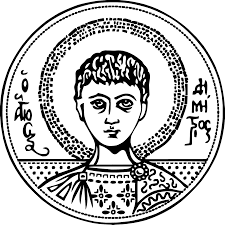
\includegraphics[height=3cm]{auth.png}\\
  \large{Αριστοτέλειο Πανεπιστήμιο Θεσσαλονίκης}\\
  \large{Τμήμα Ηλεκτρολόγων Μηχανικών Και Μηχανικών Υπολογιστών}\\
  \vspace{2cm} 
  \LARGE{Τεχνολογία Ήχου Και Εικόνας\\Κατηγοριοποίηση Καρδιακών Ήχων} 
  \vspace{3cm} 
}

\author{
  Μουστάκας Γεώργιος 9365\\
  Σαρρής Αναστάσιος Λουκάς 9451\\
  Στεφανίδης Ιωάννης 9587\\
  Σφυράκης Εμμανουήλ 9507
  \vspace{3cm}
}

\date{\today}
\newpage 

\begin{document}

\maketitle

\newpage
\tableofcontents

% Εισαγωγή
\section{Εισαγωγή}
Οι καρδιοπάθειες ταλαιπωρούν,και σε πολλές περιπτώσεις οδηγούν στον θάνατο ,ένα
μεγάλο μέρος του πληθυσμού παγκοσμίως.Η μη έγκαιρη διάγνωσή τους,η έλλειψη
εξειδικευμένου προσωπικού και σε κάποιες περιπτώσεις η έλλειψη γιατρών,είναι
κάποιες από τις αιτίες που δυσχεραίνουν αυτήν την κατάσταση.

Μία λύση στο πρόβλημα αυτό προσπάθησε να δώσει η πρόκληση του PhysioNet το
2016.Μέσα απο αυτήν,οι υπεύθυνοι ήθελαν να ενθαρρύνουν την ανάπτυξη αλγορίθμων
κατηγοριοποίησης των καρδιακών ήχων καθώς επίσης και την δημιουργία μιας μεγάλης
βάσης δεδομένων με καρδιακούς ήχους.Ο σκοπός είναι μέσα από ένα μικρό δείγμα
ήχου(10 με 60 δευτερόλεπτα),μέσω του αλγορίθμου,να διαχωρίζεται ο ήχος σε
φυσιολογικό ή μη φυσιολογικό,οπότε και χρειάζεται να διαγνωστεί από κάποιον
ειδικό.


% Καρδιακοί Ήχοι
\section{Καρδιακοί ήχοι}

Κατά τη διάρκεια του καρδιακού κύκλου,η καρδιά παράγει ηλεκτρική δραστηριότητα,
η οποία στη συνέχεια προκαλεί κολπικές και κοιλιακές συσπάσεις. Αυτό με την
σειρά του οδηγεί το αίμα γύρω από το σώμα. Το άνοιγμα και το κλείσιμο των
καρδιακών βαλβίδων σχετίζεται με επιταχύνσεις-επιβραδύνσεις του αίματος,
προκαλώντας δονήσεις ολόκληρης της καρδιακής δομής. Αυτές οι δονήσεις ακούγονται
στα θωρακικά τοιχώματα και η ακρόαση συγκεκριμένων καρδιακών ήχων μπορεί να
δώσει μια ένδειξη για την υγεία της καρδιάς. Το φωνοκαρδιογράφημα (PCG) είναι η
γραφική αναπαράσταση μιας εγγραφής καρδιακού ήχου.Ένα τυπικό PCG φαίνεται στην
παρακάτω εικόνα:

\begin{figure}[H]
	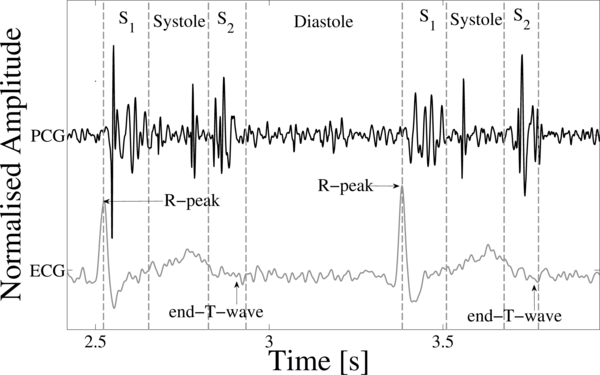
\includegraphics[width=\textwidth]{pcg.png}
	\caption{PCG και ECG \cite{clifford2016classification}}
	\label{PCG}
\end{figure}

Όπως φαίνεται και στην εικόνα ένας πλήρης καρδιακός κύκλος στο φωνοκαρδιογράφημα
αποτελείται από τέσσερις διακριτές περιοχές.Αυτές είναι οι S1, συστολή, S2 και
διαστολή.Και οι τέσσερις ήχοι που αποτελούν ένα κύκλο σχετίζονται με το κλείσιμο
συγκεκριμένων βαλβίδων και την ροή αίματος από και πρός τις κοιλίες. \cite{physionet}


% Η προσέγγιση μας
\section{Η προσέγγισή μας}\label{our_approach}

Η προσέγγισή μας έχει 3 βασικά μέρη:
\begin{itemize}
	\item \textbf{Κατάτμηση} των PCG δειγμάτων στις βασικές περιοχές του καρδιακού
	      ήχου.
	\item \textbf{MFCC μετασχηματισμό} των PCG δειγμάτων σε αναπαράσταση
	      χρόνου-συχνότητας της κατανομής της ενέργειας του σήματος.
	\item \textbf{Εκπαίδευση \& Κατηγοροποίηση} των MFCC heat maps με την χρήση
	      του συνελικτικού νευρωνικού δικτύου.
\end{itemize}

\subsection{Κατάτμηση Δειγμάτων}

Για να κάνουμε την κατάτμηση των PCG δειγμάτων όπως φαίνεται στην εικόνα
\ref{PCG} θα χρησιμοποιήσουμε των αλγόριθμο του Springer
\cite{springer2015logistic} τον οποίο τον παρείχε ο διαγωνισμός στους
συμμετέχοντες. Ωστόσο δεν θα χρησιμοποιήσουμε όλα τα δεδομένα που μας δίνει ο
αλγόριθμος, αλλά αυτό που θα κάνουμε είναι να βρίσκουμε που ξεκινάει το πρώτο
\emph{S1} και στη συνέχεια θα αναλύουμε τα 3 επόμενα δευτερόλεπτα. Αυτή η
διαδικασία θα γίνεται ώστε τα δείγματα με τα οποία θα εκπαιδεύσουμε το νευρονικό
δίκτυο να είναι ``ευθυγραμισμένα'' μεταξύ τους.


\subsection{Μετασχησματισμός MFCC}

Αφού πάρουμε τα 3 δευτερόλεπτα σκοπός είναι να δημιουργήσουμε μια εικόνα που θα
απεικονίζει χαρακτηριστικά του ηχητικού αποσπάσματος ώστε να μπορέσουμε να
προπονήσουμε το νευρωνικό μας δίκτυο. Αυτό μπορούμε να το πετύχουμε
υπολογίζοντας τις MFCC τιμές του καρδιογραφήματος με την εξής διαδικασία:

\begin{enumerate}
	\item Παίρνουμε επικαλυπτόμενα παράθυρα πάνω στο ηχητικό δείγμα
	\item Υπολογίζουμε τον μετασχηματισμό Fourier για κάθε παράθυρο
	\item Εφαρμόζουμε τα Mel φίλτρα και αθροίζουμε τις ενέργειες σε κάθε φίλτρο
	\item Υπολογίζουμε τις λογαριθμικές τιμές των παραπάνω ενεργειών
	\item Τέλος παίρνουμε τον διακριτό συνημιτονικό μετασχηματισμό των λογαριθμικών
	      τιμών.
\end{enumerate}

Έτσι θα έχουμε 12 MFCC τιμές για κάθε παράθυρο και μαζί με την ολική ενέργεια
του παραθύρου ως ξεχωριστή τιμή παίρνουμε 13 τιμές. Αναπαριστώντας αυτά τα
χαρακτηριστικά σε ένα γράφημα όπου ο $y$ άξονας θα κυμαίνετε από 0 εώς 12 (μία
γραμμή για κάθε MFCC τιμή) και ο $x$ άξονας από 0 εώς $3000 / step\_size$
(\emph{step\_size} που θα ορίσουμε για κάθε παράθυρο), θα πάρουμε ένα heat map
(βλέπε \ref{mfcc}) που μπορούμε να χρησιμοποιήσουμε ως εικόνα για το νευρωνικό
δίκτυο.

\begin{figure}[H]
	\center
	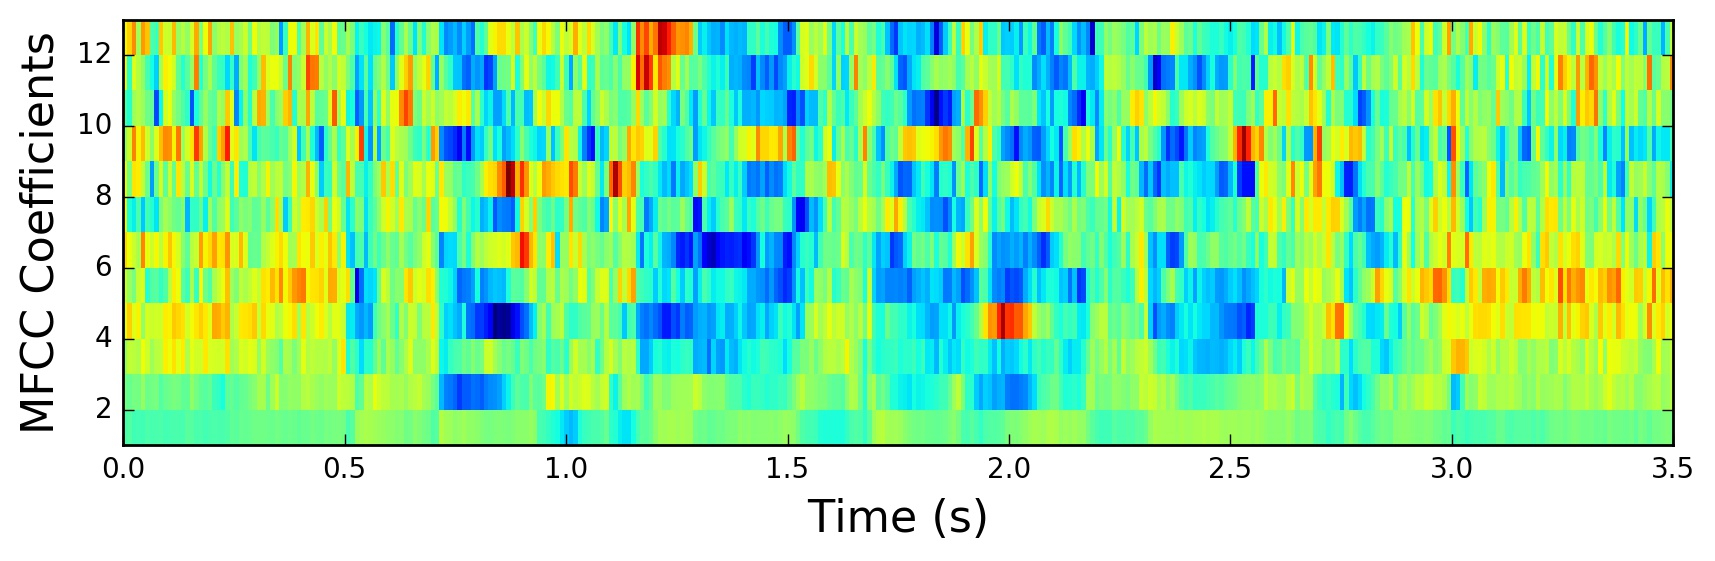
\includegraphics[width=0.7\textwidth]{mfcc.jpeg}
	\caption{MFCC heat map \cite{fayek2016}}
	\label{mfcc}
\end{figure}

\subsection{Νευρωνικό δίκτυο}

Η μετατροπή των δοθέντων μονοδιάστατων χρονοσειρών σε πίνακες θερμότητας δύο διαστάσεων
μας επιτρέπει την επεξεργασία δειγμάτων των καρδιακών ήχων υπό τη μορφή εικόνας. Γι' αυτό
κρίνεται και επιβεβλημένη η χρήση συνελικτικών νευρωνικών δικτύων λόγω των αυξανόμενων
δυνατοτήτων τους στην ανάλυση εικόνων.
\subsubsection{Αρχιτεκτονική δικτύου}

Το νευρωνικό δίκτυο δέχεται σαν είσοδο ένα κανάλι 13x300 MFCC χάρτη θερμότητας
(αν χρησιμοποιήσουμε βήμα 10ms στον MFCC μετασχηματισμό) και δίνει σαν τελική
έξοδο την ζητούμενη δυαδική κατηγοριοποίηση. Ενδιάμεσα χρησιμοποιούνται δύο
συνελικτικά στρώματα, το καθένα ακολουθούμενο από ένα στρώμα max-pooling, και
συνολικά ακολουθούμενο από δύο πλήρως συνδεδεμένα κρυφά στρώματα. \par

Το πρώτο συνελικτικό στρώμα μαθαίνει 64 2x20 πυρήνες,χρησιμοποιώντας την τεχνική
same-padding.  Στη συνέχεια εφαρμόζουμε ένα max-pooling φίλτρο
1x20,χρησιμοποιώντας ένα οριζόντιο βήμα μήκους 5, το οποίο έχει ως αποτέλεσμα τη
μείωση των διαστάσεων καθενός από τους 64 χάρτες χαρακτηριστικών σε 13x60. Ένα
δεύτερο συνελικτικό στρώμα χρησιμοποιεί 64 πυρήνες 2x10 επάνω στο προηγούμενο
στρώμα,ξανά με same-padding.Μετά την προαναφερθείσα διαδικασία ακολουθεί και
πάλι η διαδικασία max-pooling,με την χρήση φίλτρου 1x4 και βήματος 2,μειώνοντας
με αυτό τον τρόπο τη διάσταση του χάρτη χαρακτηριστικών σε 13x30.Ακολουθεί μια
διαδικασία πλάτυνσης για την μετατροπή καθενός από τους 64 13x30 χάρτες
χαρακτηριστικών σε διάνυσμα μεγέθους 24,960. Το διάνυσμα αυτό εισάγεται στο
πρώτο πλήρως συνδεδεμένο κρυφό στρώμα μήκους 1024 κρυφών μονάδων
και,ακολουθούμενο από ένα δεύτερο κρυφό στρώμα 512 κρυφών μονάδων,δίνει την
δυαδική έξοδο κατηγοριοποίησης. \par

\begin{figure}[H]
	\center
	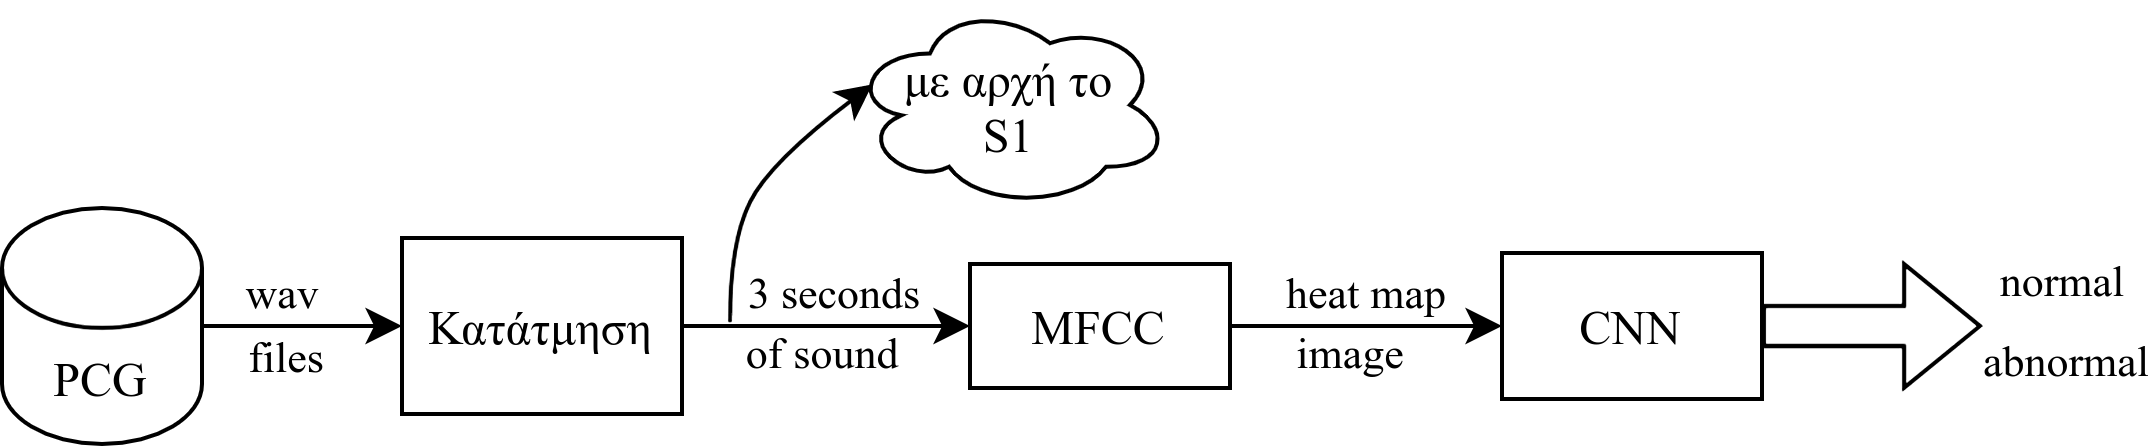
\includegraphics[width=\textwidth]{hear_sound_classification_diagram.png}
	\caption{Διάγραμμα της προσέγγισής μας για την κατηγοροποίηση καρδικών ήχων}
	\label{our_approach_diagram}
\end{figure}


% Εργαλεία
\section{Εργαλεία}
Στην προσπάθεια μας αυτή,η γλώσσα προγραμματισμού με την οποία θα δουλέψουμε
είναι η Python .Η βασική βιβλιοθήκη λογισμικού που θα χρησιμοποιήσουμε είναι το
Tensor Flow.Πρόκειται, για μια συμβολική βιβλιοθήκη μαθηματικών και
χρησιμοποιείται, επίσης, για εφαρμογές μηχανικής μάθησης, όπως νευρωνικά δίκτυα.
Επίσης, σε κάποια σημεία θα εργαστούμε και με το Matlab.


% Αποτελέσματα
\documentclass[../main.tex]{subfiles}
\graphicspath{{\subfix{../images/}}}

\begin{document}

Στα παρακάτω σχήματα φαίνονται τρις σημαντικές μετρικές που καταγράφαμε κατά την
διάρκεια της εκπαίδευσης.

Πρώτη είναι η μετρική \textbf{Accuracy} που μας δείχνει πόσο συχνά οι προβλέψεις
του νευρωνικού δικτύου είναι σωστές.

Δεύτερη είναι η μετρική \textbf{Loss} και πιο συγκεκριμένα στα σχήματα
\ref{mfcc_loss} και \ref{spectogram_recall} χρησιμοποιήσαμε την \textit{Binary
	crossentropy loss function} η οποία υπολογίζει πόσο απέχει η πρόβλεψη του
νευρωνικού από την πραγματική τιμή μέσω της παρακάτω συνάρτησης
\ref{eq:binary_crossentropy}.

\begin{equation}\label{eq:binary_crossentropy}
	\mathrm{Loss} = - \frac{1}{\mathrm{output \atop size}} \sum_{i=1}^{\mathrm{output \atop size}} y_i \cdot \mathrm{log}\; {\hat{y}}_i + (1-y_i) \cdot \mathrm{log}\; (1-{\hat{y}}_i)
\end{equation}

Τελευταία μετρική είναι η \textbf{Recall} την οποία θεωρήσαμε πολύ σημαντική για
το συγκεκριμένο πρόβλημα, καθώς μας δείχνει το ποσοστό των σωστά
κατηγοροποιημένων ατόμων με πρόβλημα, από το σύνολο όλων αυτών τον ατόμων
(ιδανικά θα θέλαμε να έχουμε 100\% recall, δηλαδή να μπορούμε να εντοπίσουμε
κάθε άτομο με καρδιακό πρόβλημα).

\subsection{Χρήση MFCC}

Με την χρήση των MFCC ως είσοδο στο νευρωνικό το accuracy σταθεροποιείται κοντά
στο 81\%, ενώ το validation\_loss έχει αρκετή απόκλιση από το loss και κυμαίνετε
ανάμεσα στο 0.4 με 0.5. Το recall έχει δραματικές μεταβολές από εποχή σε εποχή
κάτι που θα εξηγηθεί παρακάτω, με μια μέση τιμή 45\% μετά την
40\textsuperscript{στη} εποχή.

\begin{figure}[H]
	\center
	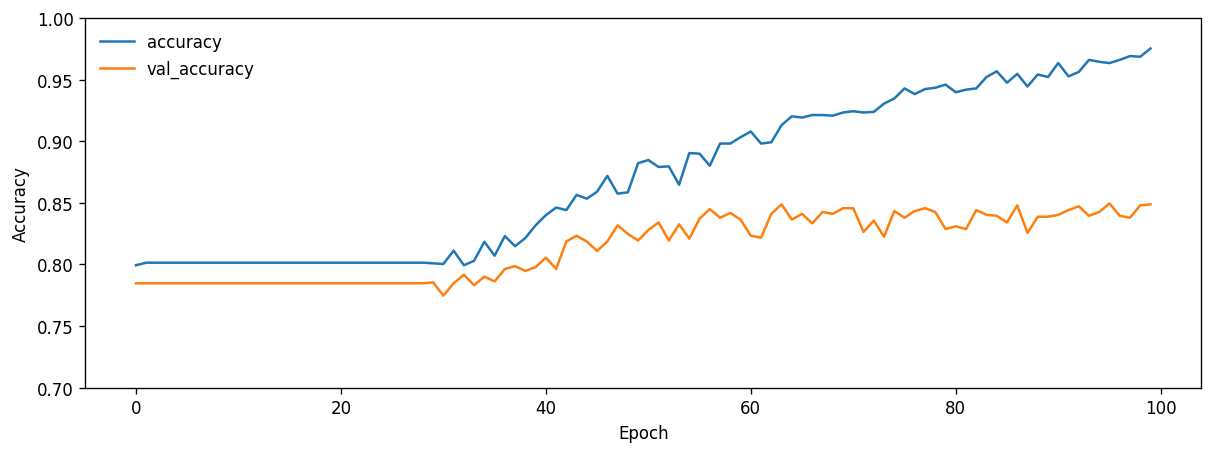
\includegraphics[width=\textwidth]{../images/mfcc_accuracy.png}
	\caption{Accuracy νευρωνικού δικτύου ανά εποχή με χρήση \textbf{MFCCs} ως
		είσοδο}
	\label{mfcc_accuracy}
\end{figure}
\begin{figure}[H]
	\center
	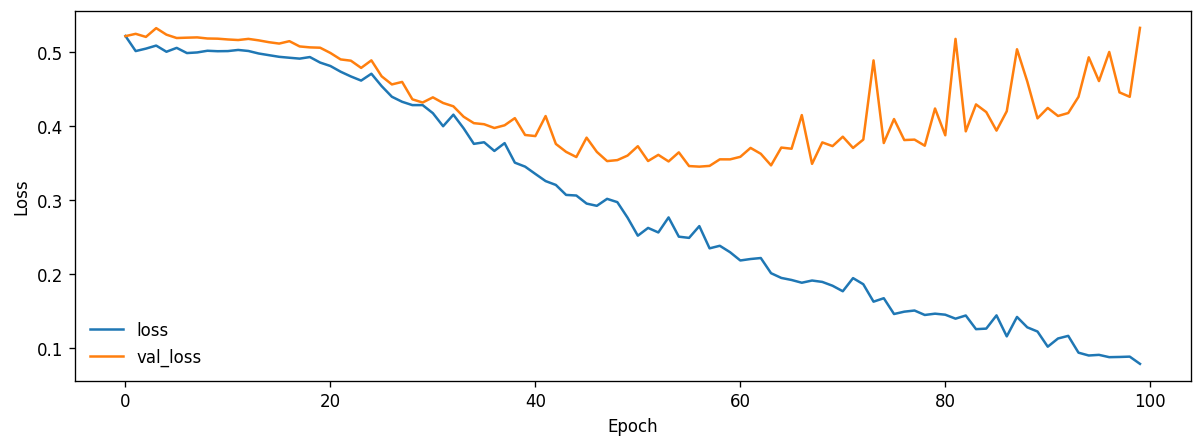
\includegraphics[width=\textwidth]{../images/mfcc_loss.png}
	\caption{Loss νευρωνικού δικτύου ανά εποχή με χρήση \textbf{MFCCs} ως
		είσοδο}
	\label{mfcc_loss}
\end{figure}
\begin{figure}[H]
	\center
	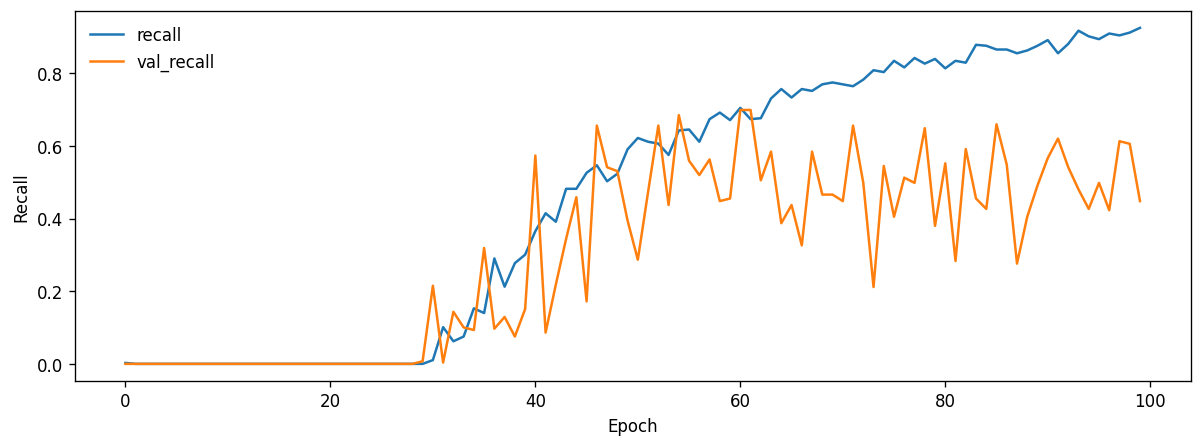
\includegraphics[width=\textwidth]{../images/mfcc_recall.png}
	\caption{Recall νευρωνικού δικτύου ανά εποχή με χρήση \textbf{MFCCs} ως
		είσοδο}
	\label{mfcc_recall}
\end{figure}


\subsection{Χρήση Mel spectogram}

Όταν χρησιμοποιήσαμε τα mel σπεκτογράμματα ως είσοδο στο νευρωνικό δίκτυο,
είδαμε ελαφρώς καλύτερα αποτελέσματα. Αφού πλέον η ακρίβεια σταθεροποιείται στο
86\% και το validation\_loss δεν απέχει τόσο από το loss με μέση τιμή κάτω από
0.35. Όσο αναφορά το recall, έχουμε κι εδώ μεγάλες μεταβολές από εποχή σε εποχή
με την τιμή να βρίσκετε γύρω από το 57\%.

\begin{figure}[H]
	\center
	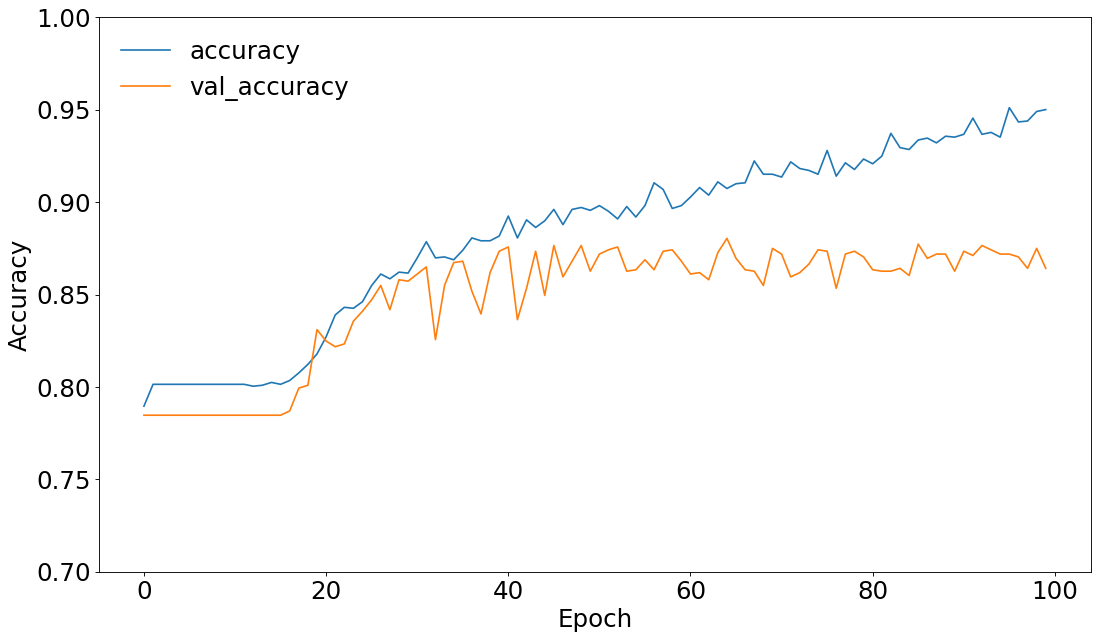
\includegraphics[width=\textwidth]{../images/spectogram_accuracy.png}
	\caption{Accuracy νευρωνικού δικτύου ανά εποχή με χρήση \textbf{spectogram} ως
		είσοδο}
	\label{spectogram_accuracy}
\end{figure}
\begin{figure}[H]
	\center
	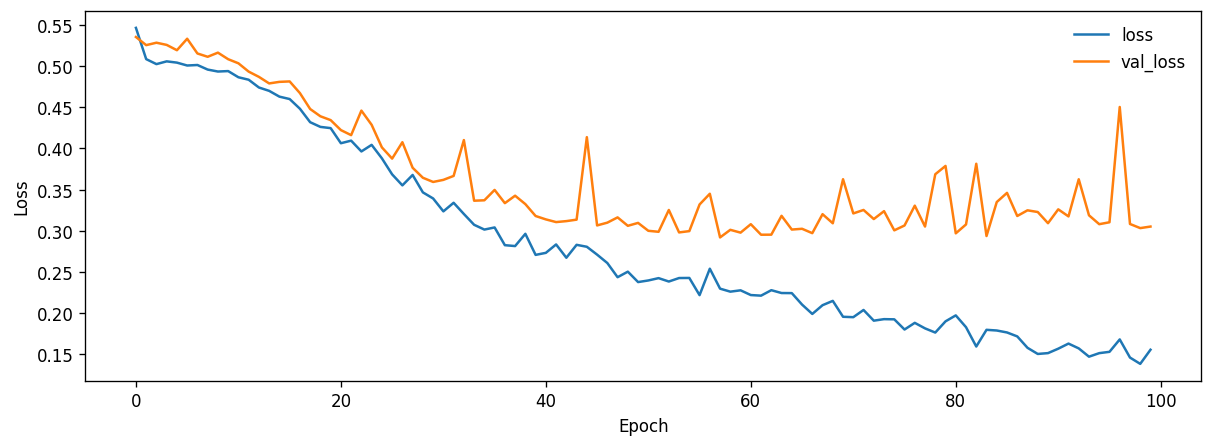
\includegraphics[width=\textwidth]{../images/spectogram_loss.png}
	\caption{Loss νευρωνικού δικτύου ανά εποχή με χρήση \textbf{spectogram} ως
		είσοδο}
	\label{spectogram_loss}
\end{figure}
\begin{figure}[H]
	\center
	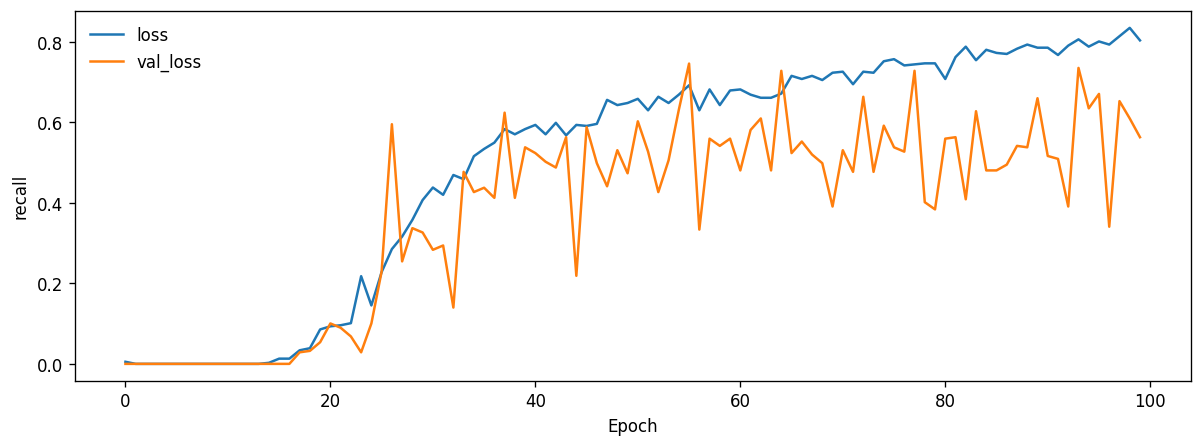
\includegraphics[width=\textwidth]{../images/spectogram_recall.png}
	\caption{Recall νευρωνικού δικτύου ανά εποχή με χρήση \textbf{spectogram} ως
		είσοδο}
	\label{spectogram_recall}
\end{figure}

\subsection{Συμπεράσματα}

Όπως είδαμε παραπάνω η καλύτερη προσπάθεια μας είχε 86\% accuracy με 57\% recall
όμως ακόμα κι αυτή η προσπάθεια δεν είναι ικανοποιητική λόγω των άνισων
δεδομένων. Τα δείγματα που παρείχε η Physionet \cite{physionet} ήταν συνολικά
3228 από τα οποία μόνο τα 665 (20\%) ήταν από ανθρώπους με καρδιοπάθεια.
Αυτό σημαίνει ότι ακόμα κι ένα νευρωνικό που θα κατηγοροποιούσε όλα τα δείγματα
ως 0 (δηλαδή χωρίς καρδιοπάθεια) θα είχε accuracy περίπου 80\% αλλά με 0\%
recall. Αυτή είναι και η αιτία που βλέπουμε και τις μεγάλες μεταβολές από εποχή
σε εποχή στο recall καθώς το δίκτυο έχει την τάση να κατηγοριοποιεί κάθε δείγμα
ως άτομο χωρίς καρδιοπάθεια λόγω της αριθμητικής υπεροχής αυτών τον ατόμων στα
δείγματα.

\end{document}


% Συζήτηση
\section{Συζητηση}


\end{document}
